\documentclass{standalone}
\usepackage{tikz}
\usetikzlibrary{patterns, positioning}

\begin{document}
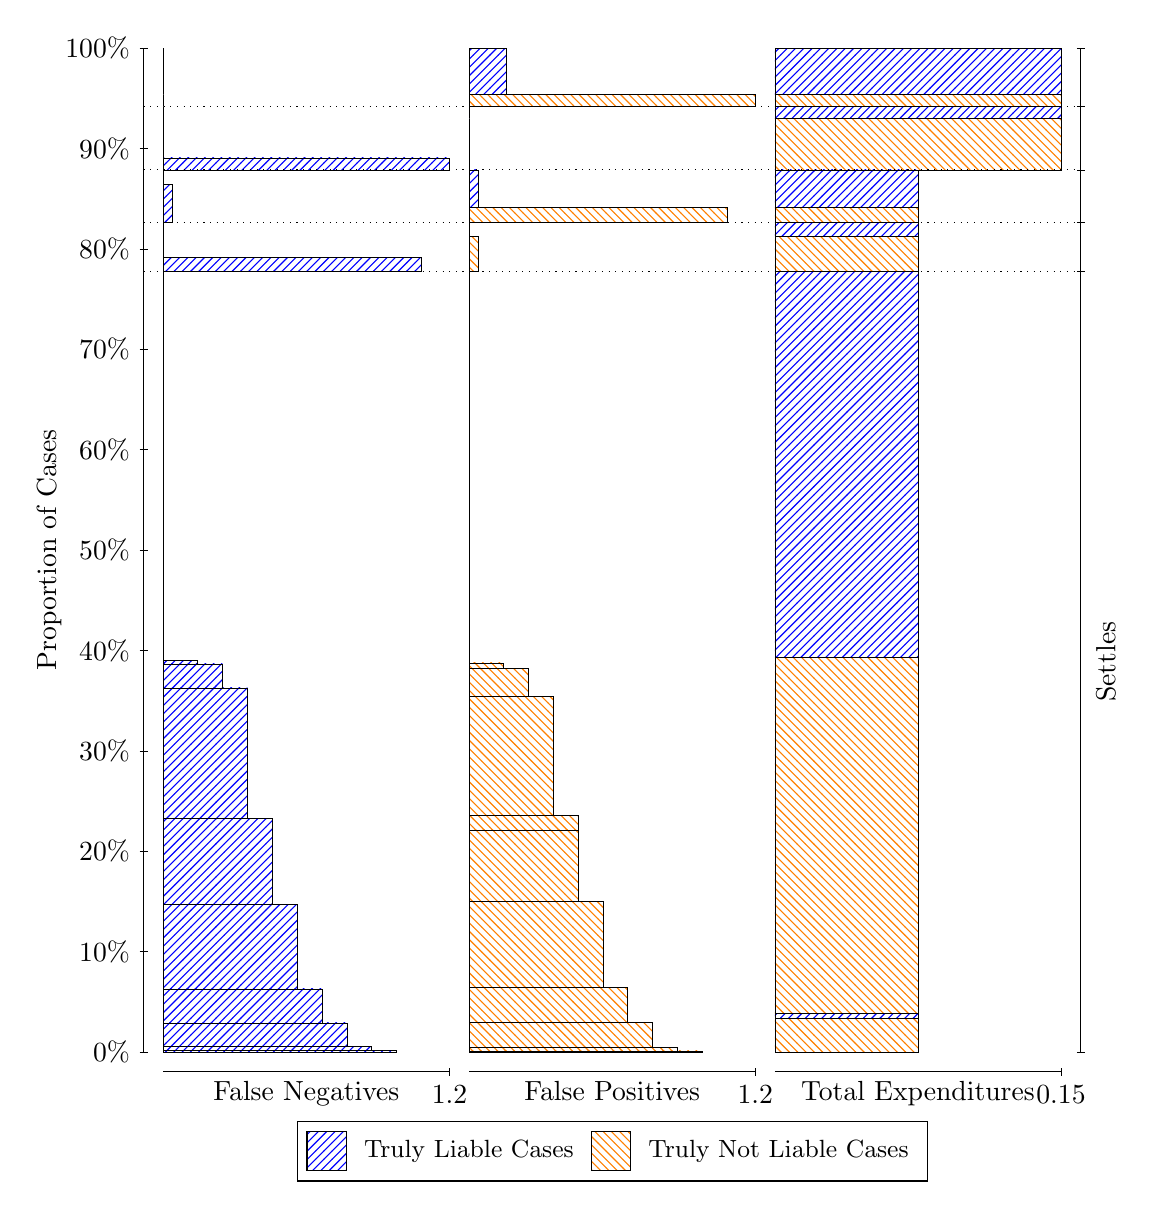
\begin{tikzpicture}
\draw[black, very thin] (1.5,1.75) -- (1.5,14.5);
\node[rotate=90, anchor=center] at (0.3, 8.125) {Proportion of Cases};
\draw[black, very thin] (1.45,1.75) -- (1.55,1.75);
\node[anchor=east] at (1.45, 1.75) {0\%};
\draw[black, very thin] (1.45,3.025) -- (1.55,3.025);
\node[anchor=east] at (1.45, 3.025) {10\%};
\draw[black, very thin] (1.45,4.3) -- (1.55,4.3);
\node[anchor=east] at (1.45, 4.3) {20\%};
\draw[black, very thin] (1.45,5.575) -- (1.55,5.575);
\node[anchor=east] at (1.45, 5.575) {30\%};
\draw[black, very thin] (1.45,6.85) -- (1.55,6.85);
\node[anchor=east] at (1.45, 6.85) {40\%};
\draw[black, very thin] (1.45,8.125) -- (1.55,8.125);
\node[anchor=east] at (1.45, 8.125) {50\%};
\draw[black, very thin] (1.45,9.4) -- (1.55,9.4);
\node[anchor=east] at (1.45, 9.4) {60\%};
\draw[black, very thin] (1.45,10.675) -- (1.55,10.675);
\node[anchor=east] at (1.45, 10.675) {70\%};
\draw[black, very thin] (1.45,11.95) -- (1.55,11.95);
\node[anchor=east] at (1.45, 11.95) {80\%};
\draw[black, very thin] (1.45,13.225) -- (1.55,13.225);
\node[anchor=east] at (1.45, 13.225) {90\%};
\draw[black, very thin] (1.45,14.5) -- (1.55,14.5);
\node[anchor=east] at (1.45, 14.5) {100\%};

\draw[black, very thin] (13.4,1.75) -- (13.4,14.5);
\draw[black, very thin] (13.35,1.75) -- (13.45,1.75);
\node[anchor=west] at (13.35, 1.75) {};
\draw[black, very thin] (13.35,11.664) -- (13.45,11.664);
\node[anchor=west] at (13.35, 11.664) {};
\draw[black, very thin] (13.35,12.288) -- (13.45,12.288);
\node[anchor=west] at (13.35, 12.288) {};
\draw[black, very thin] (13.35,12.953) -- (13.45,12.953);
\node[anchor=west] at (13.35, 12.953) {};
\draw[black, very thin] (13.35,13.759) -- (13.45,13.759);
\node[anchor=west] at (13.35, 13.759) {};
\draw[black, very thin] (13.35,14.5) -- (13.45,14.5);
\node[anchor=west] at (13.35, 14.5) {};

\draw[black, very thin, pattern color=blue, pattern=north east lines] (1.75,1.75) rectangle (4.712,1.7682);
\draw[black, very thin, pattern color=blue, pattern=north east lines] (1.75,1.7682) rectangle (4.396,1.8187);
\draw[black, very thin, pattern color=blue, pattern=north east lines] (1.75,1.8187) rectangle (4.0801,2.1193);
\draw[black, very thin, pattern color=blue, pattern=north east lines] (1.75,2.1193) rectangle (3.7641,2.5526);
\draw[black, very thin, pattern color=blue, pattern=north east lines] (1.75,2.5526) rectangle (3.4482,3.6274);
\draw[black, very thin, pattern color=blue, pattern=north east lines] (1.75,3.6274) rectangle (3.1322,4.7146);
\draw[black, very thin, pattern color=blue, pattern=north east lines] (1.75,4.7146) rectangle (2.8163,6.3743);
\draw[black, very thin, pattern color=blue, pattern=north east lines] (1.75,6.3743) rectangle (2.5004,6.6786);
\draw[black, very thin, pattern color=blue, pattern=north east lines] (1.75,6.6786) rectangle (2.1844,6.7238);
\draw[black, very thin, pattern color=orange, pattern=north west lines] (1.75,6.7238) rectangle (1.75,11.664);
\draw[black, very thin, pattern color=blue, pattern=north east lines] (1.75,11.664) rectangle (5.0279,11.845);
\draw[black, very thin, pattern color=orange, pattern=north west lines] (1.75,11.845) rectangle (1.75,12.288);
\draw[black, very thin, pattern color=blue, pattern=north east lines] (1.75,12.288) rectangle (1.8685,12.767);
\draw[black, very thin, pattern color=orange, pattern=north west lines] (1.75,12.767) rectangle (1.75,12.953);
\draw[black, very thin, pattern color=blue, pattern=north east lines] (1.75,12.953) rectangle (5.3833,13.106);
\draw[black, very thin, pattern color=orange, pattern=north west lines] (1.75,13.106) rectangle (1.75,13.759);
\draw[black, very thin, pattern color=orange, pattern=north west lines] (1.75,13.759) rectangle (1.75,13.911);
\draw[black, very thin, pattern color=blue, pattern=north east lines] (1.75,13.911) rectangle (1.75,14.5);
\draw[black, very thin, pattern color=orange, pattern=north west lines] (5.6333,1.75) rectangle (8.5953,1.7632);
\draw[black, very thin, pattern color=orange, pattern=north west lines] (5.6333,1.7632) rectangle (8.2793,1.8056);
\draw[black, very thin, pattern color=orange, pattern=north west lines] (5.6333,1.8056) rectangle (7.9634,2.1215);
\draw[black, very thin, pattern color=orange, pattern=north west lines] (5.6333,2.1215) rectangle (7.6475,2.5664);
\draw[black, very thin, pattern color=orange, pattern=north west lines] (5.6333,2.5664) rectangle (7.3315,3.6578);
\draw[black, very thin, pattern color=orange, pattern=north west lines] (5.6333,3.6578) rectangle (7.0156,4.5711);
\draw[black, very thin, pattern color=orange, pattern=north west lines] (5.6333,4.5711) rectangle (7.0156,4.7519);
\draw[black, very thin, pattern color=orange, pattern=north west lines] (5.6333,4.7519) rectangle (6.6996,6.2677);
\draw[black, very thin, pattern color=orange, pattern=north west lines] (5.6333,6.2677) rectangle (6.3837,6.6171);
\draw[black, very thin, pattern color=orange, pattern=north west lines] (5.6333,6.6171) rectangle (6.0678,6.6904);
\draw[black, very thin, pattern color=blue, pattern=north east lines] (5.6333,6.6904) rectangle (5.6333,11.664);
\draw[black, very thin, pattern color=orange, pattern=north west lines] (5.6333,11.664) rectangle (5.7518,12.107);
\draw[black, very thin, pattern color=blue, pattern=north east lines] (5.6333,12.107) rectangle (5.6333,12.288);
\draw[black, very thin, pattern color=orange, pattern=north west lines] (5.6333,12.288) rectangle (8.9112,12.475);
\draw[black, very thin, pattern color=blue, pattern=north east lines] (5.6333,12.475) rectangle (5.7518,12.953);
\draw[black, very thin, pattern color=orange, pattern=north west lines] (5.6333,12.953) rectangle (5.6333,13.606);
\draw[black, very thin, pattern color=blue, pattern=north east lines] (5.6333,13.606) rectangle (5.6333,13.759);
\draw[black, very thin, pattern color=orange, pattern=north west lines] (5.6333,13.759) rectangle (9.2667,13.911);
\draw[black, very thin, pattern color=blue, pattern=north east lines] (5.6333,13.911) rectangle (6.1072,14.5);
\draw[black, very thin, pattern color=orange, pattern=north west lines] (9.5167,1.75) rectangle (11.333,2.1727);
\draw[black, very thin, pattern color=blue, pattern=north east lines] (9.5167,2.1727) rectangle (11.333,2.2414);
\draw[black, very thin, pattern color=orange, pattern=north west lines] (9.5167,2.2414) rectangle (11.333,6.7591);
\draw[black, very thin, pattern color=blue, pattern=north east lines] (9.5167,6.7591) rectangle (11.333,11.664);
\draw[black, very thin, pattern color=orange, pattern=north west lines] (9.5167,11.664) rectangle (11.333,12.107);
\draw[black, very thin, pattern color=blue, pattern=north east lines] (9.5167,12.107) rectangle (11.333,12.288);
\draw[black, very thin, pattern color=orange, pattern=north west lines] (9.5167,12.288) rectangle (11.333,12.475);
\draw[black, very thin, pattern color=blue, pattern=north east lines] (9.5167,12.475) rectangle (11.333,12.953);
\draw[black, very thin, pattern color=orange, pattern=north west lines] (9.5167,12.953) rectangle (13.15,13.606);
\draw[black, very thin, pattern color=blue, pattern=north east lines] (9.5167,13.606) rectangle (13.15,13.759);
\draw[black, very thin, pattern color=orange, pattern=north west lines] (9.5167,13.759) rectangle (13.15,13.911);
\draw[black, very thin, pattern color=blue, pattern=north east lines] (9.5167,13.911) rectangle (13.15,14.5);
\draw[black, dotted] (1.5,11.664) -- (13.4,11.664);
\draw[black, dotted] (1.5,12.288) -- (13.4,12.288);
\draw[black, dotted] (1.5,12.953) -- (13.4,12.953);
\draw[black, dotted] (1.5,13.759) -- (13.4,13.759);
\draw[black, very thin] (1.75,1.5) -- (5.3833,1.5);
\node[anchor=north] at (3.5667, 1.5) {False Negatives};
\draw[black, very thin] (5.3833,1.45) -- (5.3833,1.55);
\node[anchor=north] at (5.3833, 1.45) {1.2};

\draw[black, very thin] (5.6333,1.5) -- (9.2667,1.5);
\node[anchor=north] at (7.45, 1.5) {False Positives};
\draw[black, very thin] (9.2667,1.45) -- (9.2667,1.55);
\node[anchor=north] at (9.2667, 1.45) {1.2};

\draw[black, very thin] (9.5167,1.5) -- (13.15,1.5);
\node[anchor=north] at (11.333, 1.5) {Total Expenditures};
\draw[black, very thin] (13.15,1.45) -- (13.15,1.55);
\node[anchor=north] at (13.15, 1.45) {0.15};

\node[black, centered, rotate=90] at (13.72, 6.7071) {Settles};





\draw (7.449999999999999,1.5) node[draw=none] (baseCoordinate) {};
\begin{scope}[align=center]
        \matrix[scale=0.5, draw=black, below=0.5cm of baseCoordinate, nodes={draw}, column sep=0.1cm]{
            \node[rectangle, draw, minimum width=0.5cm, minimum height=0.5cm, pattern=north east lines, pattern color=blue] {}; &
            \node[draw=none, font=\small] (B) {Truly Liable Cases}; &
            \node[rectangle, draw, minimum width=0.5cm, minimum height=0.5cm, pattern=north west lines, pattern color=orange] {}; &
            \node[draw=none, font=\small] (B) {Truly Not Liable Cases}; \\
            };
\end{scope}

\end{tikzpicture}
\end{document}